\documentclass{standalone}
\usepackage{tikz}
\usetikzlibrary{patterns, positioning}
\usepackage[sfdefault]{ClearSans} %% option 'sfdefault' activates Clear Sans as the default text font
\usepackage[T1]{fontenc}

\begin{document}
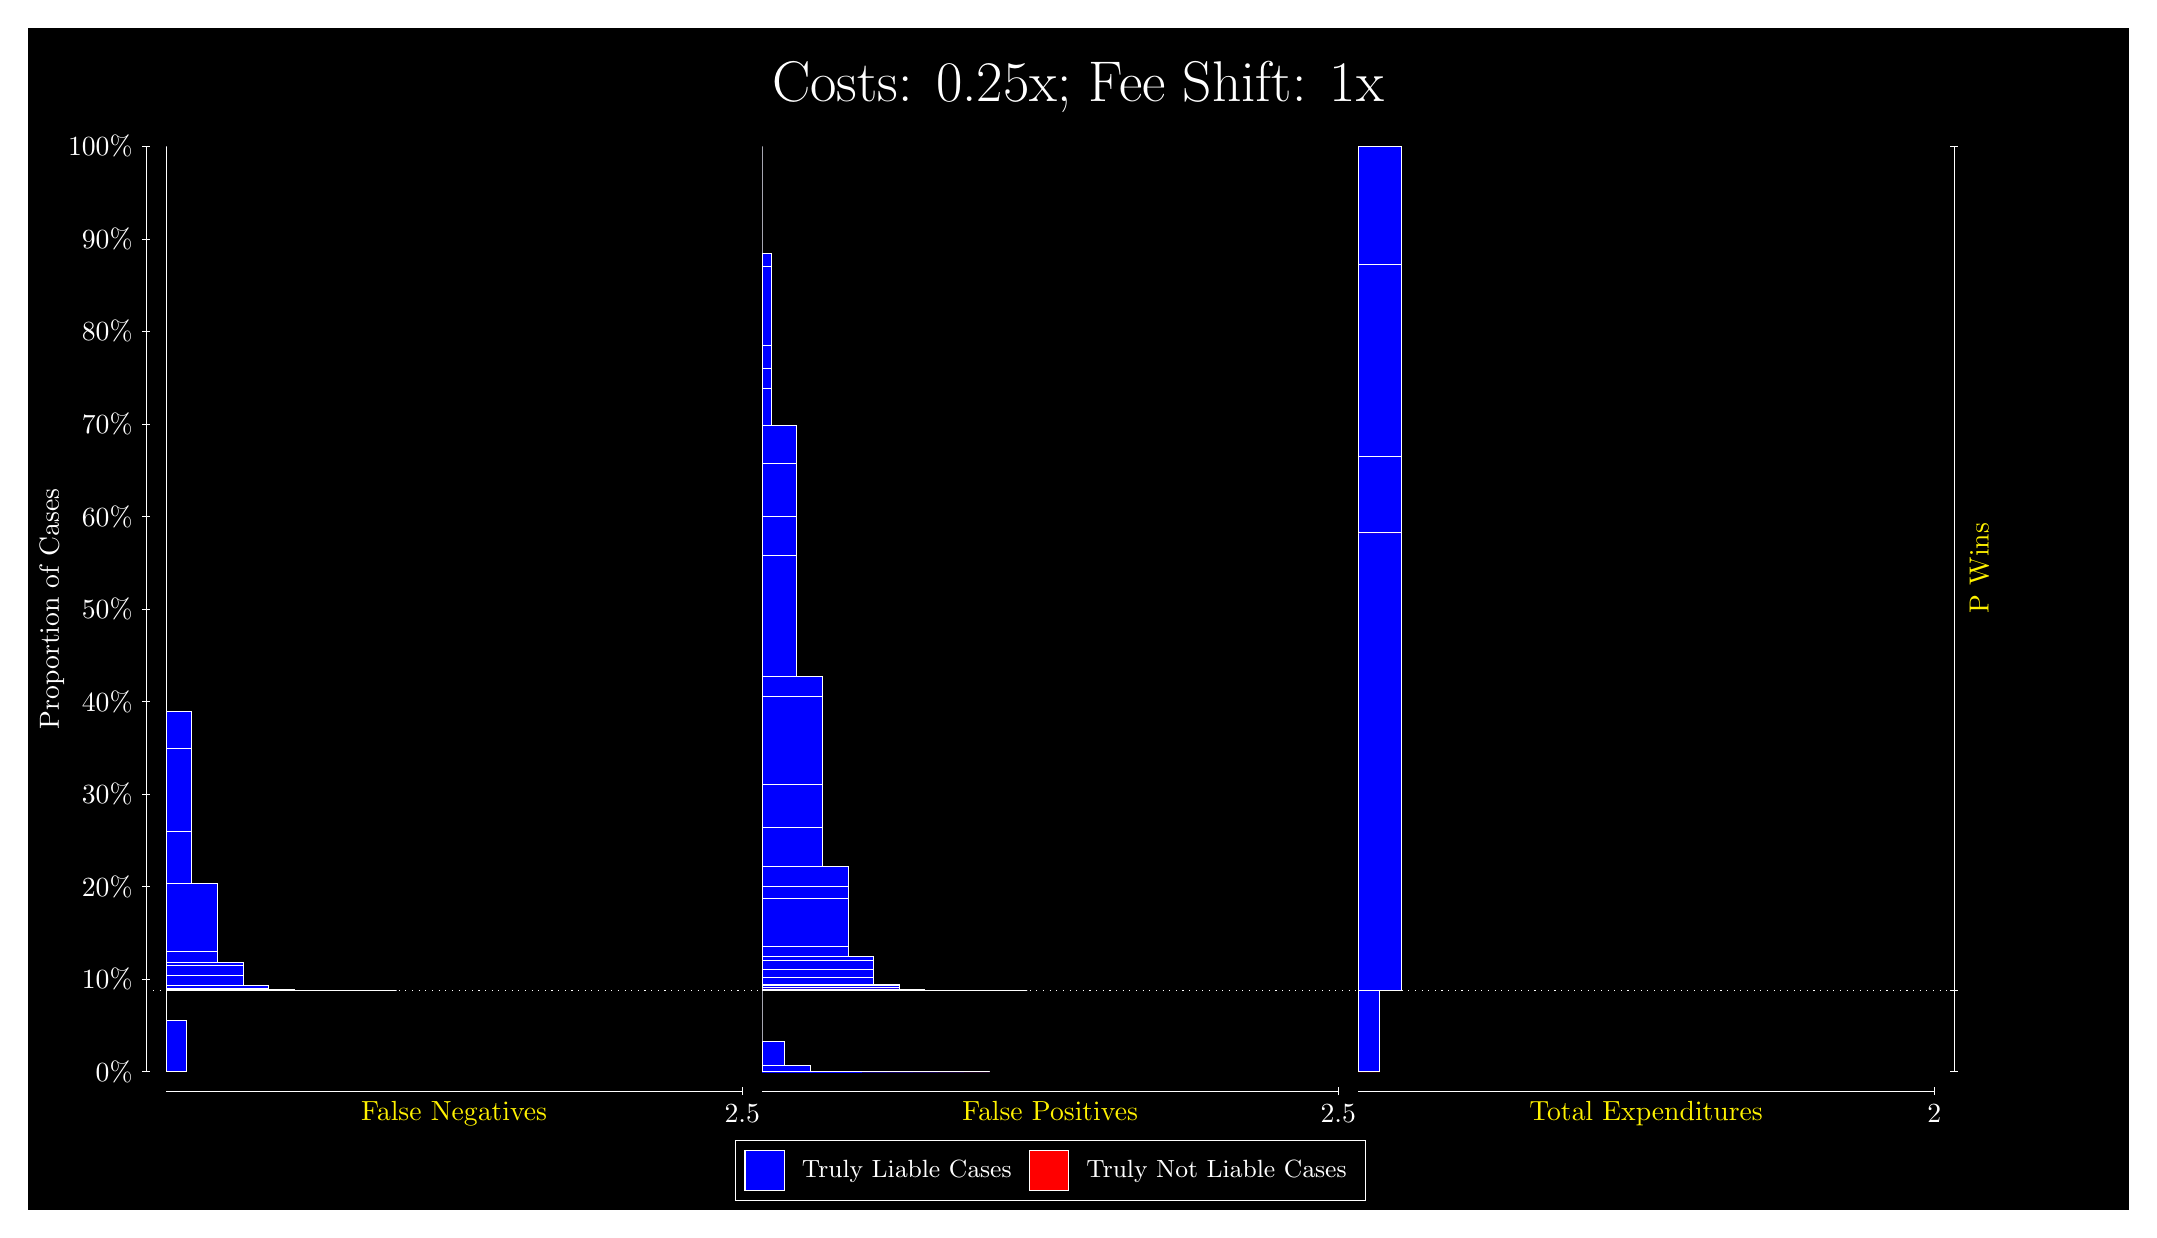
\begin{tikzpicture}
\draw[fill=black] (0,0) rectangle (26.667,15);
\draw[text=white] (0,13.5) rectangle (26.667,15) node[midway] {\huge Costs: 0.25x; Fee Shift: 1x};
\draw[white, very thin] (1.5,1.75) -- (1.5,13.5);
\node[rotate=90, text=white, anchor=center] at (0.3, 7.625) {Proportion of Cases};
\draw[white, very thin] (1.45,1.75) -- (1.55,1.75);
\node[text=white, anchor=east] at (1.45, 1.75) {0\%};
\draw[white, very thin] (1.45,2.925) -- (1.55,2.925);
\node[text=white, anchor=east] at (1.45, 2.925) {10\%};
\draw[white, very thin] (1.45,4.1) -- (1.55,4.1);
\node[text=white, anchor=east] at (1.45, 4.1) {20\%};
\draw[white, very thin] (1.45,5.275) -- (1.55,5.275);
\node[text=white, anchor=east] at (1.45, 5.275) {30\%};
\draw[white, very thin] (1.45,6.45) -- (1.55,6.45);
\node[text=white, anchor=east] at (1.45, 6.45) {40\%};
\draw[white, very thin] (1.45,7.625) -- (1.55,7.625);
\node[text=white, anchor=east] at (1.45, 7.625) {50\%};
\draw[white, very thin] (1.45,8.8) -- (1.55,8.8);
\node[text=white, anchor=east] at (1.45, 8.8) {60\%};
\draw[white, very thin] (1.45,9.975) -- (1.55,9.975);
\node[text=white, anchor=east] at (1.45, 9.975) {70\%};
\draw[white, very thin] (1.45,11.15) -- (1.55,11.15);
\node[text=white, anchor=east] at (1.45, 11.15) {80\%};
\draw[white, very thin] (1.45,12.325) -- (1.55,12.325);
\node[text=white, anchor=east] at (1.45, 12.325) {90\%};
\draw[white, very thin] (1.45,13.5) -- (1.55,13.5);
\node[text=white, anchor=east] at (1.45, 13.5) {100\%};

\draw[white, very thin] (24.457,1.75) -- (24.457,13.5);
\draw[white, very thin] (24.407,1.75) -- (24.507,1.75);
\node[anchor=west] at (24.407, 1.75) {};
\draw[white, very thin] (24.407,2.7841) -- (24.507,2.7841);
\node[anchor=west] at (24.407, 2.7841) {};
\draw[white, very thin] (24.407,13.5) -- (24.507,13.5);
\node[anchor=west] at (24.407, 13.5) {};

\draw[white, very thin, fill=blue] (1.75,1.75) rectangle (2.0062,2.4007);
\draw[white, very thin, fill=red] (1.75,2.4007) rectangle (1.75,2.4007);
\draw[white, very thin, fill=blue] (1.75,2.4007) rectangle (1.75,2.7841);
\draw[white, very thin, fill=blue] (1.75,2.7841) rectangle (4.6775,2.7841);
\draw[white, very thin, fill=blue] (1.75,2.7841) rectangle (4.3523,2.7841);
\draw[white, very thin, fill=blue] (1.75,2.7841) rectangle (4.027,2.7841);
\draw[white, very thin, fill=blue] (1.75,2.7841) rectangle (4.027,2.7841);
\draw[white, very thin, fill=blue] (1.75,2.7841) rectangle (3.7017,2.7843);
\draw[white, very thin, fill=blue] (1.75,2.7843) rectangle (3.7017,2.7846);
\draw[white, very thin, fill=blue] (1.75,2.7846) rectangle (3.3764,2.7912);
\draw[white, very thin, fill=blue] (1.75,2.7912) rectangle (3.0511,2.8109);
\draw[white, very thin, fill=blue] (1.75,2.8109) rectangle (3.0511,2.8467);
\draw[white, very thin, fill=blue] (1.75,2.8467) rectangle (2.7258,2.9669);
\draw[white, very thin, fill=blue] (1.75,2.9669) rectangle (2.7258,3.1015);
\draw[white, very thin, fill=blue] (1.75,3.1015) rectangle (2.7258,3.1408);
\draw[white, very thin, fill=blue] (1.75,3.1408) rectangle (2.4006,3.2712);
\draw[white, very thin, fill=blue] (1.75,3.2712) rectangle (2.4006,4.1362);
\draw[white, very thin, fill=blue] (1.75,4.1362) rectangle (2.0753,4.8037);
\draw[white, very thin, fill=blue] (1.75,4.8037) rectangle (2.0753,5.8563);
\draw[white, very thin, fill=blue] (1.75,5.8563) rectangle (2.0753,6.3231);
\draw[white, very thin, fill=red] (1.75,6.3231) rectangle (1.75,6.3231);
\draw[white, very thin, fill=blue] (1.75,6.3231) rectangle (1.75,13.5);
\draw[white, very thin, fill=red] (9.3189,1.75) rectangle (12.21,1.75);
\draw[white, very thin, fill=blue] (9.3189,1.75) rectangle (12.21,1.75);
\draw[white, very thin, fill=blue] (9.3189,1.75) rectangle (11.885,1.75);
\draw[white, very thin, fill=blue] (9.3189,1.75) rectangle (11.559,1.75);
\draw[white, very thin, fill=blue] (9.3189,1.75) rectangle (11.234,1.75);
\draw[white, very thin, fill=blue] (9.3189,1.75) rectangle (10.909,1.75);
\draw[white, very thin, fill=blue] (9.3189,1.75) rectangle (10.583,1.7503);
\draw[white, very thin, fill=blue] (9.3189,1.7503) rectangle (10.258,1.7573);
\draw[white, very thin, fill=blue] (9.3189,1.7573) rectangle (9.9328,1.829);
\draw[white, very thin, fill=blue] (9.3189,1.829) rectangle (9.6076,2.1333);
\draw[white, very thin, fill=blue] (9.3189,2.1333) rectangle (9.3189,2.7841);
\draw[white, very thin, fill=red] (9.3189,2.7841) rectangle (12.686,2.7841);
\draw[white, very thin, fill=blue] (9.3189,2.7841) rectangle (12.686,2.7841);
\draw[white, very thin, fill=red] (9.3189,2.7841) rectangle (12.36,2.7841);
\draw[white, very thin, fill=blue] (9.3189,2.7841) rectangle (12.36,2.7841);
\draw[white, very thin, fill=red] (9.3189,2.7841) rectangle (12.035,2.7841);
\draw[white, very thin, fill=blue] (9.3189,2.7841) rectangle (12.035,2.7841);
\draw[white, very thin, fill=blue] (9.3189,2.7841) rectangle (12.035,2.7841);
\draw[white, very thin, fill=blue] (9.3189,2.7841) rectangle (12.035,2.7841);
\draw[white, very thin, fill=red] (9.3189,2.7841) rectangle (11.71,2.7841);
\draw[white, very thin, fill=blue] (9.3189,2.7841) rectangle (11.71,2.7846);
\draw[white, very thin, fill=blue] (9.3189,2.7846) rectangle (11.71,2.7848);
\draw[white, very thin, fill=red] (9.3189,2.7848) rectangle (11.384,2.7848);
\draw[white, very thin, fill=blue] (9.3189,2.7848) rectangle (11.384,2.7886);
\draw[white, very thin, fill=blue] (9.3189,2.7886) rectangle (11.384,2.7932);
\draw[white, very thin, fill=blue] (9.3189,2.7932) rectangle (11.059,2.815);
\draw[white, very thin, fill=red] (9.3189,2.815) rectangle (11.059,2.815);
\draw[white, very thin, fill=blue] (9.3189,2.815) rectangle (11.059,2.8413);
\draw[white, very thin, fill=blue] (9.3189,2.8413) rectangle (11.059,2.8612);
\draw[white, very thin, fill=blue] (9.3189,2.8612) rectangle (10.734,2.9527);
\draw[white, very thin, fill=blue] (9.3189,2.9527) rectangle (10.734,3.0508);
\draw[white, very thin, fill=red] (9.3189,3.0508) rectangle (10.734,3.0508);
\draw[white, very thin, fill=blue] (9.3189,3.0508) rectangle (10.734,3.1664);
\draw[white, very thin, fill=blue] (9.3189,3.1664) rectangle (10.734,3.2111);
\draw[white, very thin, fill=blue] (9.3189,3.2111) rectangle (10.409,3.3426);
\draw[white, very thin, fill=red] (9.3189,3.3426) rectangle (10.409,3.3426);
\draw[white, very thin, fill=blue] (9.3189,3.3426) rectangle (10.409,3.9469);
\draw[white, very thin, fill=blue] (9.3189,3.9469) rectangle (10.409,4.1017);
\draw[white, very thin, fill=blue] (9.3189,4.1017) rectangle (10.409,4.361);
\draw[white, very thin, fill=blue] (9.3189,4.361) rectangle (10.083,4.8576);
\draw[white, very thin, fill=blue] (9.3189,4.8576) rectangle (10.083,5.4021);
\draw[white, very thin, fill=red] (9.3189,5.4021) rectangle (10.083,5.4021);
\draw[white, very thin, fill=blue] (9.3189,5.4021) rectangle (10.083,6.5211);
\draw[white, very thin, fill=blue] (9.3189,6.5211) rectangle (10.083,6.7654);
\draw[white, very thin, fill=blue] (9.3189,6.7654) rectangle (9.758,8.3126);
\draw[white, very thin, fill=red] (9.3189,8.3126) rectangle (9.758,8.3126);
\draw[white, very thin, fill=blue] (9.3189,8.3126) rectangle (9.758,8.7992);
\draw[white, very thin, fill=blue] (9.3189,8.7992) rectangle (9.758,9.4737);
\draw[white, very thin, fill=blue] (9.3189,9.4737) rectangle (9.758,9.961);
\draw[white, very thin, fill=blue] (9.3189,9.961) rectangle (9.4327,10.428);
\draw[white, very thin, fill=blue] (9.3189,10.428) rectangle (9.4327,10.678);
\draw[white, very thin, fill=blue] (9.3189,10.678) rectangle (9.4327,10.972);
\draw[white, very thin, fill=blue] (9.3189,10.972) rectangle (9.4327,11.973);
\draw[white, very thin, fill=blue] (9.3189,11.973) rectangle (9.4327,12.148);
\draw[white, very thin, fill=blue] (9.3189,12.148) rectangle (9.3189,13.5);
\draw[white, very thin, fill=red] (16.888,1.75) rectangle (17.162,1.75);
\draw[white, very thin, fill=blue] (16.888,1.75) rectangle (17.162,2.7841);
\draw[white, very thin, fill=red] (16.888,2.7841) rectangle (17.437,2.7841);
\draw[white, very thin, fill=blue] (16.888,2.7841) rectangle (17.437,8.5935);
\draw[white, very thin, fill=red] (16.888,8.5935) rectangle (17.437,8.5935);
\draw[white, very thin, fill=blue] (16.888,8.5935) rectangle (17.437,9.5679);
\draw[white, very thin, fill=red] (16.888,9.5679) rectangle (17.437,9.5679);
\draw[white, very thin, fill=blue] (16.888,9.5679) rectangle (17.437,12.003);
\draw[white, very thin, fill=red] (16.888,12.003) rectangle (17.437,12.003);
\draw[white, very thin, fill=blue] (16.888,12.003) rectangle (17.437,13.5);
\draw[white, dotted] (1.5,2.7841) -- (24.457,2.7841);
\draw[white, very thin] (1.75,1.5) -- (9.0689,1.5);
\node[text=yellow, anchor=north] at (5.4094, 1.5) {False Negatives};
\draw[white, very thin] (9.0689,1.45) -- (9.0689,1.55);
\node[text=white, anchor=north] at (9.0689, 1.45) {2.5};

\draw[white, very thin] (9.3189,1.5) -- (16.638,1.5);
\node[text=yellow, anchor=north] at (12.978, 1.5) {False Positives};
\draw[white, very thin] (16.638,1.45) -- (16.638,1.55);
\node[text=white, anchor=north] at (16.638, 1.45) {2.5};

\draw[white, very thin] (16.888,1.5) -- (24.207,1.5);
\node[text=yellow, anchor=north] at (20.547, 1.5) {Total Expenditures};
\draw[white, very thin] (24.207,1.45) -- (24.207,1.55);
\node[text=white, anchor=north] at (24.207, 1.45) {2};


\node[text=yellow, centered, rotate=90] at (24.777, 8.142) {P Wins};

\draw (12.978300999999998,1.5) node[draw=none] (baseCoordinate) {};
\begin{scope}[align=center]
        \matrix[scale=0.5, draw=white, below=0.5cm of baseCoordinate, nodes={draw}, column sep=0.1cm]{
            \node[rectangle, draw, minimum width=0.5cm, minimum height=0.5cm, fill=blue] {}; &
            \node[draw=none, font=\small, text=white] (B) {Truly Liable Cases}; &
            \node[rectangle, draw, minimum width=0.5cm, minimum height=0.5cm, fill=red] {}; &
            \node[draw=none, font=\small, text=white] (B) {Truly Not Liable Cases}; \\
            };
\end{scope}

\end{tikzpicture}
\end{document}